%%%%%%%%%%%%%%%%%%%%%%%%%%%%%%%%%%%%%%%%%%%%%%%%%%%%%%%%%%%%%%%%%%%%%%%%%%%%%%%%%%%%%%%%%%%%%%%%%%%%%%%%%%%%%%%%%%%%%%%%%%%%%%%%%%%%%%%%%%%%%%%%%%%%%%%%%%%%%%%%%%%
% Written By Michael Brodskiy
% Class: Fundamentals of Networks
% Professor: E. Bernal Mor
%%%%%%%%%%%%%%%%%%%%%%%%%%%%%%%%%%%%%%%%%%%%%%%%%%%%%%%%%%%%%%%%%%%%%%%%%%%%%%%%%%%%%%%%%%%%%%%%%%%%%%%%%%%%%%%%%%%%%%%%%%%%%%%%%%%%%%%%%%%%%%%%%%%%%%%%%%%%%%%%%%%

\documentclass[12pt]{article} 
\usepackage{alphalph}
\usepackage[utf8]{inputenc}
\usepackage[russian,english]{babel}
\usepackage{titling}
\usepackage{amsmath}
\usepackage{graphicx}
\usepackage{enumitem}
\usepackage{amssymb}
\usepackage[super]{nth}
\usepackage{everysel}
\usepackage{ragged2e}
\usepackage{geometry}
\usepackage{multicol}
\usepackage{fancyhdr}
\usepackage{cancel}
\usepackage{siunitx}
\usepackage{physics}
\usepackage{tikz}
\usepackage{mathdots}
\usepackage{yhmath}
\usepackage{cancel}
\usepackage{color}
\usepackage{array}
\usepackage{multirow}
\usepackage{gensymb}
\usepackage{tabularx}
\usepackage{extarrows}
\usepackage{booktabs}
\usepackage{lastpage}
\usepackage{float}
\usetikzlibrary{fadings}
\usetikzlibrary{patterns}
\usetikzlibrary{shadows.blur}
\usetikzlibrary{shapes}

\geometry{top=1.0in,bottom=1.0in,left=1.0in,right=1.0in}
\newcommand{\subtitle}[1]{%
  \posttitle{%
    \par\end{center}
    \begin{center}\large#1\end{center}
    \vskip0.5em}%

}
\usepackage{hyperref}
\hypersetup{
colorlinks=true,
linkcolor=blue,
filecolor=magenta,      
urlcolor=blue,
citecolor=blue,
}


\title{Conceptual Homework 2}
\date{October 23, 2023}
\author{Michael Brodskiy\\ \small Professor: E. Bernal Mor}

\begin{document}

\maketitle

\begin{enumerate}

  \item Do routers have IP addresses? If so, how many? If not, why?

    Yes, routers have IP addresses. The exact number depends on the router and network configuration; however, we know that there are, at the very least, two addresses. This is due to the fact that a router must have an incoming address and an outgoing address that it must differentiate between. There is no absolute maximum amount for the amount of addresses a router may have, but there are many factors which can limit it, such as: quantity of allocated addresses to a network and hardware of a router (CPU, RAM, etc.).

  \item Suppose an application generates chunks of 960 bytes of data, and each chunk gets encapsulated in a TCP segment and then an IPv4 packet (no optional header fields). What percentage of each packet will be overhead (including transport and network layer), and what percentage will be application data?

  \item Suppose a router has four links, numbered 0 through 3. Destination-based forwarded is used and the forwarding table is given by:

    \begin{center}
      \begin{tabular}[h!]{|c|c|c|}
        \hline
        Entry & Destination Address & Output Link Interface\\
        \hline
        1 & 11100000 00****** ******** ******** & 0\\
        \hline
        2 & 11100000 01000000 ******** ******** & 1\\
        \hline
        3 & 1110000* ******** ******** ******** & 2\\
        \hline
        4 & 11100001 1******* ******** ******** & 3\\
        \hline
        5 & Otherwise & 4\\
        \hline
      \end{tabular}
    \end{center}

  Obtain the appropriate output link interface for the datagrams with the following destination addresses. \underline{Explain how you reached your answer and include the interface and} \underline{the table entry chosen}

    \begin{enumerate}

      \item 11001000 10010001 01010001 10101010 

      \item 11100001 01000000 11000011 00111100 

      \item 11100001 10000000 00010001 01110111

      \item 11100000 01000000 11001100 00011101

    \end{enumerate}

  \item What is a private network address? Should a datagram with a private network address ever be present in the larger public Internet? Explain.

  \item

    \begin{enumerate}

      \item What is meant by a control plane that is based on per-router control? are the data plane and the control plane implemented within the same devices? Briefly explain your answer.

      \item What is meant by a control plane that is based on logically centralized control? are the data plane and the control plane implemented within the same devices?Briefly explain your answer
        
    \end{enumerate}

  \item Consider the following network. With the indicated link costs, use Dijkstra’s algorithm to compute the least-cost path from $x$ to all network nodes and then obtain \underline{the resulting forwarding table}. Show how the algorithm works by \underline{computing a table }\\\underline{similar to the tables we have seen in class}.

    \begin{figure}[h]
      \centering
      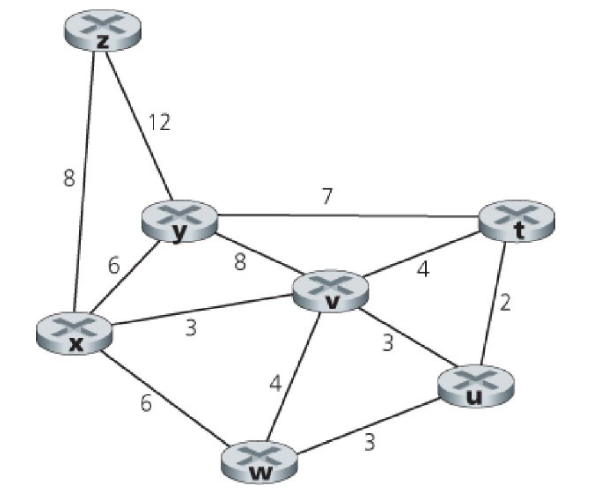
\includegraphics[width=.6\textwidth]{Figures/Djikstra.png}
      \caption{Figure for Problem 6}
      \label{fig:1}
    \end{figure}

\end{enumerate}

\end{document}

